\documentclass[USenglish,oneside,twocolumn]{article}
\usepackage{color}
\usepackage[hyphens]{url}
\usepackage{longtable}
\usepackage{graphicx}
\usepackage{enumitem}
\usepackage{pdfpages}
\usepackage{adjustbox}
%\usepackage{hyperref}

\usepackage[utf8]{inputenc}%(only for the pdftex engine)
%\RequirePackage[no-math]{fontspec}%(only for the luatex or the xetex engine)
\usepackage[big]{dgruyter_NEW}
 
\hyphenation{Isa-bela}

\DOI{foobar}

\cclogo{
\includegraphics{by-nc-nd.pdf}}

% Format a participant quotation.
\newcommand{\pquote}[2]{
\begin{quotation}
\noindent #1:~\textit{``#2''}
\end{quotation}
}
  
\begin{document}
   \author*[1]{Author 1}

  \author[2]{Author 2}

  \author[3]{Author 3}

  \author[4]{Author 4}

  \author[5]{Author 5}
  
  \author[6]{Author 6}

  \affil[1]{Affiliation of Author 1, E-mail: \mbox{author1@affiliation.edu}}
  \affil[2]{Affiliation of Author 2, E-mail: \mbox{author2@affiliation.edu}}
  \affil[3]{Affiliation of Author 3, E-mail: \mbox{author3@affiliation.edu}}
  \affil[4]{Affiliation of Author 4, E-mail: \mbox{author4@affiliation.edu}}
  \affil[5]{Affiliation of Author 5, E-mail: \mbox{author5@affiliation.edu}}
  \affil[6]{Affiliation of Author 6, E-mail: \mbox{author6@affiliation.edu}}
%  \author*[1]{Linda Lee}
%
%  \author[2]{David Fifield}
%
%  \author[3]{Nathan Malkin}
%
%  \author[4]{Ganesh Iyer}
%
%  \author[5]{Serge Egelman}
%  
%  \author[6]{David Wagner}
%
%  \affil[1]{University of California Berkeley, E-mail: \mbox{lnl@cs.berkeley.edu}}
%
%  \affil[2]{University of California Berkeley, E-mail: \mbox{fifield@cs.berkeley.edu}}
%
%  \affil[3]{University of California Berkeley, E-mail: \mbox{nmalkin@cs.berkeley.edu}}
%
%  \affil[4]{University of California Berkeley, E-mail: \mbox{ganesh.v@berkeley.edu}}
%  
%  \affil[5]{University of California Berkeley and International Computer Science Institute, E-mail: \mbox{egelman@cs.berkeley.edu}}
%   
%  \affil[6]{University of California Berkeley, E-mail: \mbox{daw@cs.berkeley.edu}}

  \title{\huge A Usability Evaluation of Tor Launcher}

  \runningtitle{A Usability Evaluation of Tor Launcher}

  %\subtitle{...}

  \begin{abstract}
{
{\color {blue}
We evaluate, design, and test the Tor Launcher interface by
placing users in simulated censorship environments, instructing them to use Tor
to circumvent censorship, and measuring their interface interactions.
A 16-participant qualitative study examines user assumptions and common mistakes.
We use the results as feedback to redesign the configuration interface.
A 114-participant quantitative study shows that our design changes result in
a significant reduction in time. We conclude with recommendations for changes 
to the current interface as well as alternative solutions.
}
}
\end{abstract}
  \keywords{Usable Security, User Studies, Tor, Security, Censorship, Anonymity}
%  \classification[PACS]{}
 % \communicated{...}
 % \dedication{...}

  \journalname{Proceedings on Privacy Enhancing Technologies}
\DOI{Editor to enter DOI}
  \startpage{1}
  \received{..}
  \revised{..}
  \accepted{..}

  \journalyear{2015}
  \journalvolume{2015}
  \journalissue{2}

\maketitle

\section{Introduction}

Tor~\cite{dingledine2004tor} is an anonymity network that routes Internet traffic through a series of relays 
that make it difficult to observe the source and destination. 
Tor Browser~\cite{torbrowser} is a modified Firefox browser with a built-in Tor client that
is the recommended way to use Tor. Tor Launcher is a Tor Browser component that
starts, stops, and otherwise controls the underlying Tor processes.
Tor Launcher's graphical user interface asks the user to configure
bridges, pluggable transports, and proxies to make a connection to Tor (we refer to this graphical user interface as the ``configuration interface'' throughout this paper). This is the object of our study. 

We hope that our work helps users more easily connect to Tor. The direct and obvious benefit of our work is that is that it may help users who would have previously been unable to configure Tor Browser to use it or that it may save time for users who would have been able to configure a valid connection to the Tor. Improving the user experience through user testing has the potential to be beneficial for both the software company (less help desk tickets) and the end users (less frustration). 

However, we believe that our work uniquely necesssary and beneficial to Tor Browser. Although originally designed for Internet anonymity, using Tor Browser to circumvent censorship has now become sufficiently common that many countries now attempt to block Tor relays for this reason~\cite{winter2012great}. Our contributions toward an easier bootstrapping process will especially benefit citizens who face Internet censorship. If there is an increase in overall users as a result, they add a security bonus by increasing the anonymity set~\cite{dingledine2006anonymity}. \\


\noindent This paper contributes:
\smallskip
\begin{itemize}
\item an evaluation of the current configuration interface
\item a redesigned configuration interface
\item logs of 114 users' connection attempts
\item failure modes seen during connection attempts
\item recommended interface changes
\item alternative bootstrapping approaches
\end{itemize}

We start by introducing relevant concepts (section~\ref{sec:background}) and
defining the scope of our experiment (section~\ref{sec:scope}). 
Then, we report user observations and interviews (section~\ref{sec:qualitative}),
list design principles and interface changes (section~\ref{redesign}),
state evaluation criteria for testing the interface (section~\ref{sec:eval}), 
and measure the impact of our design changes (Section~\ref{sec:quantitative}).
We end with a discussion on what we learned (section~\ref{sec:discussion}),
limitations of out experiment (section~\ref{sec:limitations}), 
a look at our work in the context of existing work (section~\ref{sec:related}), and
a brief conclusion (section~\ref{sec:conclusion}).

\section{Background}
\label{sec:background}
This section discusses network components involved in connecting to Tor, network conditions that require specific network components, and how to configure the involved network components. 

\subsection{Relays, Bridges, Pluggable Transports, and Proxies} 

Tor relays are routers in the Tor Network that receive and pass along Tor traffic. 
There are three types of Tor relays: guard relays that serve as an entry node, middle relays that forward traffic from an entry node to an exit node, and exit relays which directs traffic to the destination. 
Censors can block access to the Tor network by blocking these relays, which are publicly listed. 

Bridges are unlisted Tor relays that serve as an alternative entry node.
Bridges can be simple, unlisted relays. 
But most bridges run a pluggable tranport (referred to as ``transport'' for shorthand) that obfuscates the traffic. 
Most transports disguise traffic to defeat on-the-wire identification, relying on the secrecy of their static IP addresses for their effectiveness.
These include ``fte'' and ``fte-ipv6''~\cite{fte},
which disguise the Tor protocol as another protocol (such as HTTP), and
``obfs3''~\cite{obfs3}, ``obfs4''~\cite{obfs4}, and ``scramblesuit''~\cite{scramblesuit},
which encrypt or alter the Tor protocol to appear as random noise.
Some transports route traffic through other services, avoiding the need for a secret IP address. 
``flashproxy''~\cite{flashproxy} connects through third parties' web browsers,
and the ``meek''~\cite{fifield2015blocking} options route traffic
through content delivery networks.
Bridges and transports allow a connection to the Tor network when all publicly listed relays and any Tor-looking packets are blocked. Fig.~\ref{fig:bridge-options} shows the bridge and transport options at the time of the study.

\begin{figure}
  \centering
    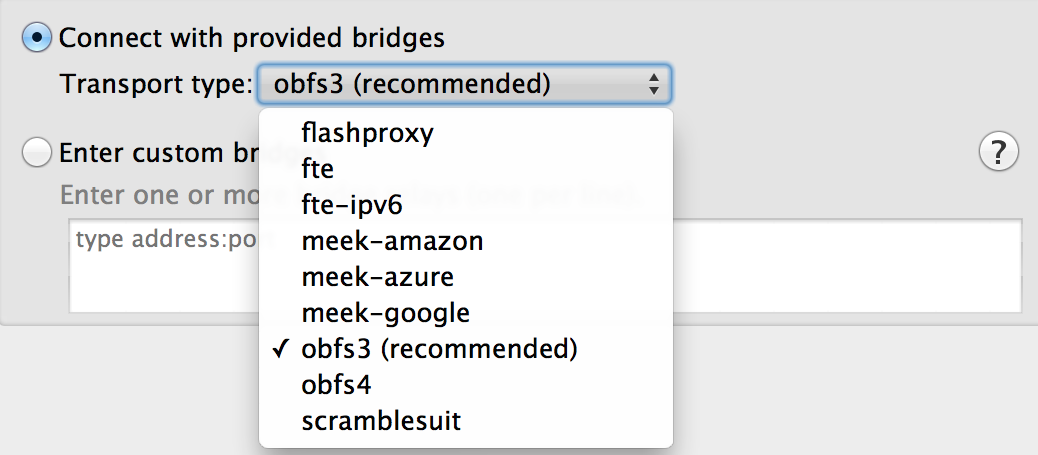
\includegraphics[width=0.5\textwidth]{bridge-options.png}
\caption{
Bridge options in Tor Browser~5.0.3's Tor Launcher interface.
Pre-configured bridges can be selected by ``Transport type,'' which refer to various
censorship circumvention technologies (``pluggable transports'').
%Under ``Enter custom bridges,'' there is a space to paste in
%a bridge line, obtained out of band.
%The ``Help'' button displays instructions on obtaining
%bridge lines. 
}
\label{fig:bridge-options}
\end{figure}

A local proxy is required to connect 
in certain managed networks. In this paper, ``proxy'' refers to a local, ordinary unobfuscated proxy such as a SOCKS or HTTP proxy. (Technically, Tor relays, bridges, and local proxies all allow indirect network connections to other network services and can be considered a proxy.) Fig.~\ref{fig:topology} illustrates the interacting components.

\begin{figure}
\centering

\includegraphics{topology.pdf}
\caption{
The chain of components involved in connecting to a website over Tor.
Most users do not need a proxy;
only users who face a censor need a bridge.
In the diagram, ``Tor'' represents all three anonymizing hops through the Tor network.
We have shown the bridge as a separate component
because of the special role it plays.
When a bridge is used, it becomes the first Tor relay.
}
\label{fig:topology}
\end{figure}

\subsection{State and Corporate Censorship}
State level censors can vary in their thoroughness in censorship. Some block websites with a combination of IP blacklisting and DNS-poisoning while others that employ more sophisticated techniques such as deep packet inspection and protocol detection. In countries that censor services but do not block censorship circumvention tools, any connection to Tor will byass the censorship. In other countries, sophisticated state-level censorship require custom bridges or bridges that run specific tranports that route traffic through non-Tor services first. 

Some companies and educational institutions have a firewall, which can be bypassed with a proxy (with or without a connection to Tor). 

\subsection{Connecting to Tor} 
Configuring a bridge requires providing one or more
``bridge lines,'' a specifically formatted bridge specification that
includes its IP address, transport type, and other metadata.
The interface has hard-coded options (see Figure~\ref{fig:bridge-options}) 
that select a group of bridges that use a particular transport.
For instance, choosing the hard-coded obfs3 option
configures a handful of bridges that use obfs3 transport.
If the built-in bridges do not work, a user can obtain bridge lines
through out-of-band channels, for instance by email~\cite{bridgedb}.

Configuring a proxy requires providing the proxy protocol, IP address, port, and additional optional fields. The user must locate and input this information. 

There are many valid configuration settings to connect to the Tor network.
For instance, a user who needs a bridge but not need a proxy can connect to Tor with a bridge and proxy, provided that both were configured correctly. The set of valid configuration settings vary on the specific network environment. 

\section{Methodology} 
This section discusses our process, principles, and preparations for evaluating the configuration interface.

\subsection{Testing Pipeline} 
Two researchers first performed a cognitive walkthough~\cite{cognitive-walkthrough} to prepare for user testing. A cognitive walkthough is evaluation method in which usability evaluators and product experts work through a series of tasks from the perspective of the user to understand a system's learnability for new or infrequent users.

We then conducted a formative usability test~\cite{formative} that found where and why users have difficulty. Formative usability testing is a support tool designed to gain insight into how the design can be improved. 5 users is considered to be user testing's maximum benefit-cost ratio for gaining insights~\cite{howmanyusers}, so we recruited for 5 participants in each experimental condition. 

Formative testing is usually used as feedback for design iterations. We opportunistically used our observations to make design changes to the configuration interface. We believed that the process of a identifying design principles, proposing design changes, and showing an alternative interface was insightful in itself---and had the potential to discover impactful changes.

We concluded with a summative usability test~\cite{summative} that determined the usability of an interface. We test the current interface to evaluate it. We also opportunistically test the redesigned interface. Summative usability testing is a quality assurance tool designed to test features in a design. In short, formative testing tells you {\it what} is or is not usable, while summative testing testing tells you {\it if} it is or is not usable. 20 users is considered to be the minimum number to statistically significant measurments~\cite{howmanyusers}, so we recruited for 20 participants in each experimental condition.  

\subsection{Evaluation Metrics}
\label{sec:eval}
Usability measures users' abilities to complete tasks. We use the following industry-standard~\cite{albert2013measuring} metrics: \\

\begin{itemize}
\item {\bfseries Completion rate:}  percentage of users that eventually connect to Tor in an experimental condition. 
\item {\bfseries Connection time:} time from Tor Browser startup to the first successful Tor bootstrap. 
\item {\bfseries Configuration time:} time spent in the Tor Launcher GUI configuring network components.
\end{itemize}

Completion rate is the fundamental usability metric that measures if users can accomplish the task. We defined success as a binary metric that is true if a user connected to Tor and false if a user did not. 

Task time is a supplemental usability metric that measures user productivity during the task. We measured task time two different ways. Connection time captured the amount of time users take to use the configuration interface to connect to Tor. This included time users spent waiting while a Tor Browser establishes a connection to Tor, which can dominate the measurement. Configuration time captured the amount of time users spent configuring bridges and proxies. 

\subsection{Experimental Setup}
\label{sec:environments}
We simulated three environments (which we refer to as E1, E2, and E3), 
which are in the order of increasing severity in censorship. Table~\ref{tab:environments} summarizes our environments and what network components are required to make a  connection to Tor. We chose to 
simulate environments for the stability, reproducibility, and simplicity of the 
experiment, as real censored networks are voilatile, subject to change, and complex. 

\begin{table}[t]
\centering
\begin{tabular}{r c c c}
& E1 & E2 & E3 \\
% \noalign{\hrule}
websites blocked & X & X & X \\
public relays blocked & & X & X \\
default bridges blocked & & & X \\
\end{tabular}
\caption{
Summary of our simulated censorship environments.
E1 only requires participants to click ``Connect'';
E2 requires a built-in bridge;
and E3 requires a specific type of built-in bridge
or manual configuration of a custom bridge.
E2's blocking is a superset of E1's;
similarly E3's is a superset of E2's.
}
\label{tab:environments}
\end{table}

The simulated environments are not intended to imitate any particular country's censorship environment. Rather, they were designed to require particular network configurations
to connect to Tor. We believe this to be sufficient for the purpose of testing the configuration interface, since these environments require the user to take the interface paths we wanted to test. 

We used features of the Windows operating system 
to block websites and Tor relays. 
We added entries to the hosts file to
mapping domain names to the address 127.0.0.1, which simulated
website by using Tor. We blocked torproject.org and its respective subdomains to discourage downloading Tor Browser, as we had installed a specific version on the test computers (E1, E2, E3).  We blocked wikipedia.org, cnn.com, and their respective subdomains to create an artificial task to visit a 
``censored'' website as motivation to connect to Tor during the experiment (E1, E2, E3). 
We specified Windows Firewall rules to block IP address of public Tor relays (E2, E3) and default bridges (E3).

For our experiments, we use versions of Tor Browser~5.0.3, 
the most recent stable release at the time~\cite{torbrowser-503}.
Though there were new releases during the experiments,
we used the same version throughout to not introduce
confounding factors.

\section{Usability Inspection}
This section discusses our inspection of the configuration interface and the resulting observations.

\subsection{Procedure} 
Two researchers performed the cognitive walkthough on the Tor Browser 5.0.3 Tor Launcher GUI, the most recent version deployed at the time (Figure~\ref{fig:old-interface}). We systematically tried action sequences from the perspective of a typical user, which we defined as a first time or infrequent user with almost no previous knowledge about network components involved in connecting to Tor.

We first examined each screen in the interface for tasks required, inputs taken, and consequences of possible actions. This was done to map all potential paths through the interface (Figure~\ref{fig:digraph}). We then stepped through each user path and recorded our observations. 

\begin{figure*}
\centering

\includegraphics[width=\textwidth]{placeholder-fullpage.pdf}
\caption{
A redesigned version of the Tor Browser 5.0.3. Tor Launcher GUI. 
}
\label{fig:old-interface}
\end{figure*} 

\subsection{Observations}
Through this process, we observed that:  \\
\begin{itemize} 
\item The interface does not presuppose that a user has previous exposure to Tor. 
\item The interface provides recommendations in text and populates options with recommended settings. 
\item The user has the burden of determining if Tor relays are blocked or if a proxy is required. 
\item A user can optionally configure a bridge and proxy even if they are not necessary to connect to Tor. 
\item Free-form inputs lead to many potential error states. 
\end{itemize} 

We used the map of potential user paths (Figure~\ref{fig:digraph}) to design our simulated environments (section~\ref{sec:environments}).  We used our walkthrough observations as inspiration for drafting our post-experiment interview questions (Appendix~\ref{interview-questions}) for formative usability testing. 

\begin{figure*}
\centering
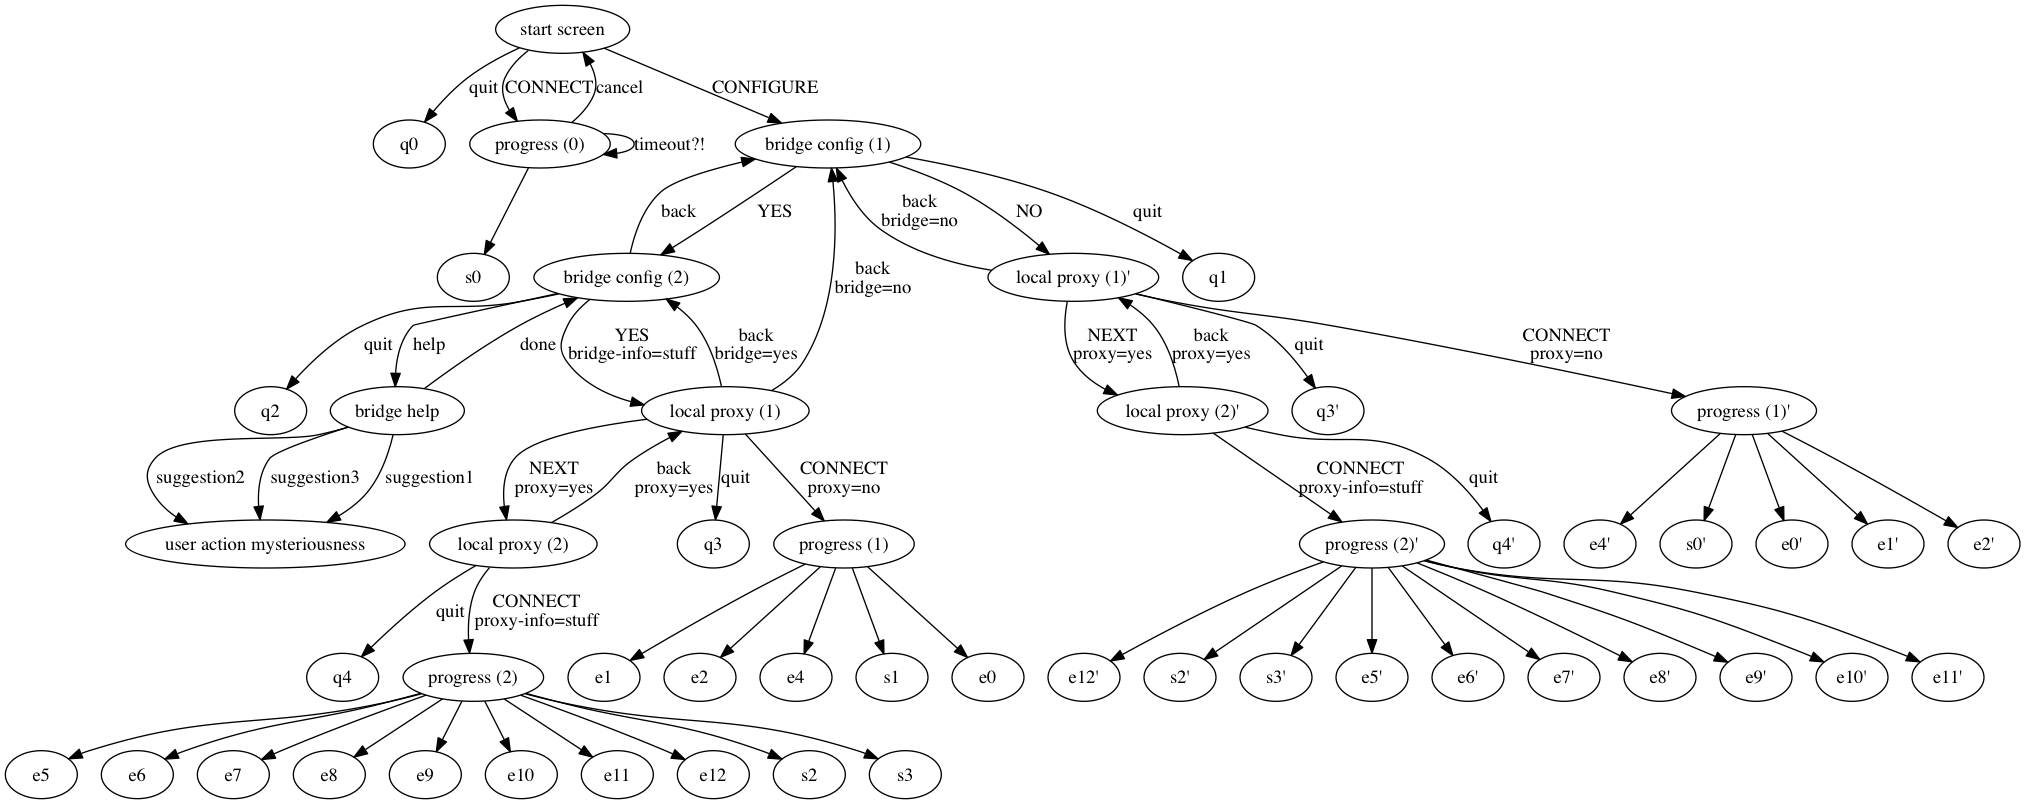
\includegraphics[width=\textwidth]{tor-digraph.png}
\caption{
A digraph illustrating the potential user paths through the interface. Non-leaf nodes are screens in the user interface (start, bridge 1, bridge 2, proxy 1, proxy 2, and progress). Leaf nodes are various end states (quit, success, or error). Tansitions between these nodes denote user actions. For details of each end state, see Appendix ~\ref{states}. 
}
\label{fig:digraph}
\end{figure*} 

\section{Formative Usability Testing}
\label{sec:qualitative}
This section discusses our small-scale, qualitative usability experiment and resulting user insights. 

\subsection{Recruitment}
We recruited people from Craigslist using the recruitment text in Appendix~\ref{qualitative-recruitment}, which linked an presecreening survey that collected demographics (Appendix~\ref{qualitative-prescreening}). We pre-screened~\cite{screening} for diversity in gender, age, technical expertise, use of security tools, and familiarity with Tor in a small participant pool. Of our 16 recruited participants, 53.3\% were male. Ages ranged from 20 to~62 years ($\mu = 24.5$, $\sigma = 12.6$). 93.3\% of our participants had college education. We took participants' self-reported familiarity with technical terms use of security tools with skepticism (Appendix~\ref{prescreening-responses}). We verified their self-reported familiarity with Tor Browser in-person, and found that 4 used it, 5 heard of it but not used it, and the remaining 8 never heard of or used it.  

We distributed participants evenly across experimental conditions:  5~in E1, 5~in E2, and 6~in E3. Although there is variation in gender, age, ``technical expertise,'' and ``use of security tools'' in each experimental condition, we ensured each condition had a participant who used Tor Browser, a participant who heard of it, and multiple participants who never heard of or used it. 

\subsection{Setup} 
We ran the experiment in a meeting room in <redacted building> at <redacted university>. The room had a desk and chair, where a monitor, keyboard, and a Windows 8 computer were set up. On a clean computer, we manually downloaded and installed the necessary software for the experiment: Tor Browser 5.0.3 for testing, Chrome, Firefox, and Internet Explorer to allow users to browse the Internet on a another browser of their choice, and VLC to record the screen during the experiment. Before each participant entered the room, we ran a script on the computer that
set up one of the three simulated environments (E1, E2, or E3) and started the screen recording.  

\subsection{Procedure}
Three researchers ran the formative usability testing, with each session having at least two researchers.  
Before the experiment began, each participant was verbally informed of the purpose of the 
study, what data was collected, and any associated risks. If they wished to participate,
they were informed again in writing and consented by signing the document. To be thorough, 
we clarified verbally that they could stop at any time during the experiment with no negative consequences. 

The experiment formally began by informing the participant of the simulated censorship environment (Appendix~\ref{qualitative-script}). This purpose of this introduction was to ensure that the main task
was to connect to Tor, rather than figuring out if they needed to connect to Tor. 
We instructed them to visit a blocked and unblocked website
in a non-Tor browser to clarify that the Internet was functioning as expected. 
We then told them to use Tor Browser to visit a censored site and pointed out 
the respective shortcut on their desktop.

We then asked them to complete a worksheet (Appendix~\ref{participant-worksheet}) that 
required answers from one blocked website (Wikipedia) and one non-blocked website (CNN).
The worksheet did not specify which website was censored. 
We chose these websites because they are popular websites and that their likely familiarity 
would make the task seem less intimidating. 

Participants were given 45 minutes to complete their worksheet. 
After instructions, the researchers left and watched a live feed of the participants' screen in another room to minimize interactions.

After participants completed the browsing tasks (or ran out of time),
we asked them standard interview questions about their experience (Appendix~\ref{interview-questions}) and took notes of their responses. We then followed up with participant-specific questions to verify any hypotheses we had from observation (e.g. ``the participant was selecting bridges at random''). We paid each participant~\$30 for their time. 

\subsection{Observations and Interviews} 
{\color {blue}
We give a summary of all participants here!  Quotations come from live transcription and are not necessarily verbatim.

Observations in E1: 
\pquote{P1, NF}{summary of what they did. ``and a quote too.''}
\pquote{P2, NF}{summary of what they did. ``and a quote too.''}
\pquote{P3, NF}{summary of what they did. ``and a quote too.''}
\pquote{P4, HT}{summary of what they did. ``and a quote too.''}
\pquote{P5, UT}{summary of what they did. ``and a quote too.''}

Observations in E2:

Observations in E3: 

\pquote{P2}{I don't know what any of those [list of bridges] means, or what that [proxy] means at all.}
\pquote{P3}{The vocabulary is really challenging, for someone not doing IT work.}
\pquote{P\#}{find when Michael said he didn't know if he was E2 or E3!} 
\pquote{P8}{I have no clue what's the difference between flashproxy, fte, etc. I need to know why the built-in ones aren't working. And why do I need a custom bridge if there are options built in?}
\pquote{P7}{Since it (obfs3) said recommended, it helped actually, and I selected it because it was chosen. I saw the custom bridges option, but I didn't know what to enter there so I went with this (obfs3).}
When participants did encounter an error message, they did not understand what errors meant (Fig.~\ref{fig:error}).
%The progress bar has a bug that causes it to update only when the level of progress increases.
%If progress bar reaches a 90\% and fails, the next attempt have regressed to 0\% and remain there until the progress surpasses 90\%. Due to this, participants assumed that their subsequent attempts were wrong, even if they were right.
\pquote{P1}{It was hard to figure out if the progress bar wasn't moving because the connection was censored, or if it was just slow.}
\pquote{P16}{There doesn't seem to be a timeout on any of this stuff. Am I waiting long enough? It should work immediately.}
\pquote{P15}{I didn't know if this computer had any proxy information. I wasn't able to find it if it did.}
}

\begin{figure}[t]
  \centering
    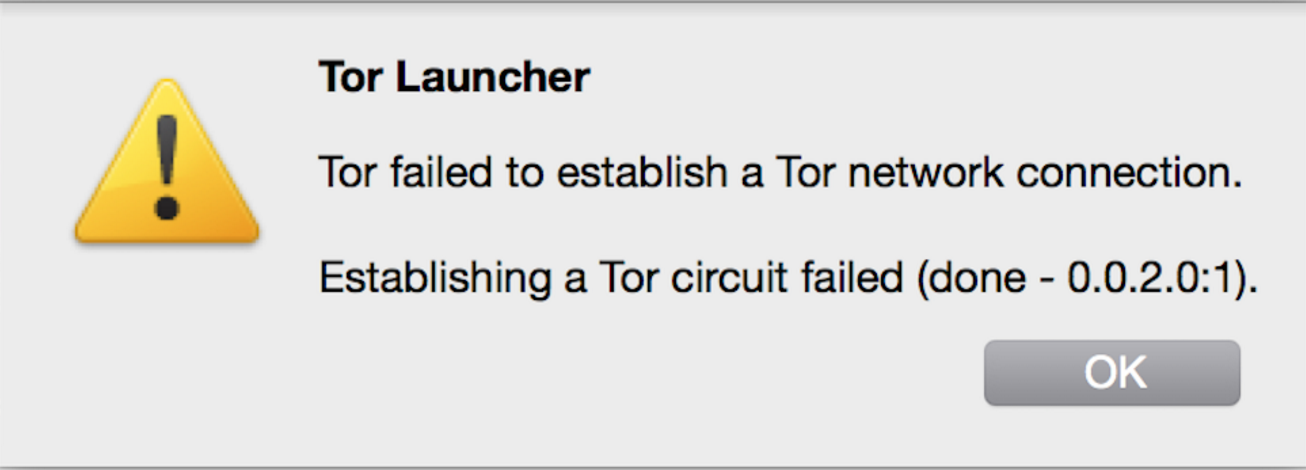
\includegraphics[width=0.5\textwidth]{error.png}
    \caption{An example of a technical error message which our participants did not understand.}
\label{fig:error}
\end{figure}

\subsection{Pain Points in Tor Launcher} 
{\color {blue}
LIST `EM! 
}

\section{A Design Iteration}
\label{sec:design} 
This section discusses how we converted our formative usability testing observations into design changes. 

\subsection{Procedure} 
Three researchers agreed on security and usability design principles. 
We then rewatched screen capture videos and read interview transcirptions to brainstorm design changes. We provided the security and usability design principles, screen capture videos, interview transcriptions, and our suggested changes to a user interface designer, who iteratively redesigned the interface with our feedback and user interface best practices in mind. Figure~\ref{fig:new-interface} shows our redesign of the interface. 

\begin{figure*}
\centering

\includegraphics[width=\textwidth]{placeholder-fullpage.pdf}
\caption{
A redesigned version of the Tor Browser 5.0.3. Tor Launcher GUI. 
}
\label{fig:new-interface}
\end{figure*} 

\subsection{Design Princples} 
The interface currently favors a guided manual configuration over an automated configuration with network probing. Our redesign preserves this approach and has no user-dependent inputs, no network-dependent inputs, and minimal information leaks.

{\color {blue} WRITE ABOUT PAIN POINTS HERE} We aimed to minimize work, give targeted feedback, and to build a mental model.

\subsection{Changes Made} 
We made these changes for a more usable interface. \\

\noindent To minimize work: 
\begin{itemize}
\item We eliminated technical questions, resulting in less tasks and interface screens. 
\item We simulated auto-detection for proxies, telling users that they did not need a proxy. This is feasible to do with a local scan (no information leaked). 
\item We labeled the configure button as an option for users in heavily censored environments.
\item We gave advice on choosing transports, telling users to try a meek bridge if obfs3 does not work.
\end{itemize} 

To give targeted feedback: 
\begin{itemize}
\item We switched added indicators to the progress bar to show the progress of bridges and proxies. 
\item We told users what to try next on errors (i.e. choose a different bridge, try a without a proxy). 
\end{itemize}

To build a mental model:
\begin{itemize}
\item We added a summary screen displays the current bridge and proxy settings for system visibility. 
\item We switched proxy and bridge screens to put them in a topologically sequential order (Figure~\ref{fig:topology}).
\end{itemize}

Figure~\ref{fig:new-interface} shows the resulting interface.  Figure~\ref{fig:old-interface} shows the unchanged version. 

\section{Summative Usability Testing}
\label{sec:quantitative}
This section discusses our large-scale quantitative usability experiment and resulting user measurements. 

\subsection{Recruitment}
We recruited  people using the recruitment text in Appendix~\ref{quantitative-recruitment}. We recruited 65 participants from Craiglist and 59 participants from the <redacted lab> participant pool. <Redacted lab> encouraged the use of their participant pool, but we bargained to recruit participants from Craigslist to ensure a diverse set of participants. Although the <redacted lab>'s participant pool is not limited to students and staff from <redacted institution>, it was estimated that a large majority were. 

Of our recruited 124 participants, 56.8\% were male. Ages ranged from 18 to~68 years ($\mu = 28.9$, $\sigma = 12$). 56.8\% were male. 84.8\% of our participants had a college education. We distributed participants evenly across experimental condition, about 20 in each interface and environment combination. Although there is variation in gender and age in each experimental condition, we ensured each condition had about half Craiglist recruited participants and half <redacted lab>  pool participants. 

\subsection{Setup}
We ran our experiment at <redacted lab>, an experimental social science laboratory for behavioral experiments. The testing room had 36 workstations with identical Windows~7 laptops. Side panels at each workstation to discouraged participants from looking at other participants' screens. 
%Xlab~\cite{xlab}, the Experimental Social Science Laboratory at the University of California, Berkeley. 
The computers at <Redacted lab> use a system restore software to revert computers to a clean version at the beginning of each session. 

Before each session, we ran a script that downloaded the necessary software, set up one of the three simulated environments (E1, E2, or E3), and downloaded the original Tor Browser 5.0.3 or a modified version of Tor Browser 5.0.3 that contained our design changes (OLD or NEW), and start the video recording. In contrast to the previous test, we installed an instrumented versions of Tor Browser 5.0.3. The instrumentation logged user interactions, such as window transitions, mouse clicks, and menu selections. Similarly to the previous test, we installed Chrome, Firefox, and Internet Explorer to allow users to browser the Internet on a browser of their choice and VLC to record the screen during the experiment. Each computer was manually assigned one of the six interface-environment combinations in a way that evenly distributed experimental conditions throughout the room and assigned an equal number of participants to each experimental condition.

\subsection{Procedure}
Participants were assigned to a computer at random, which effectively assigned them to a simulated censorship environment combination at random. Before the experiment began, participants were verbally informed of the purpose of the study, what data was collected, and any associated risks. If they wished to participate, they were ifnormed again in writing and consented by signing the document. To be thorough, we clarified that they could stop at any time during the experiment with no negative consequences. 

The experiment formally began by informing participants of the simulated censorship environment, giving them their worksheet, and informing them that Tor browser is necessary to circumvnt censorship (Appendix~\ref{quantitative-script}). This time, the worksheet only asks users to visit one blocked website (Wikipedia) and explicitly reminds users to use Tor to do so. Before participants started their tasks, we reminded them that their screens are being recorded so they should not log into anything that shows personal information. We gave users a chance to ask any questions about the experiment or task. 

Participants were given 40 minutes to complete the task. After instructions, researchers maintained minimal interactions with the participants, only answering logistical questions. Afterward, we administered an exit survey to collect demographics (Appendix~\ref{quantitative-exit-survey}). We paid each participant \$30 for their time. 

\subsection{Results} 
124 people participated in our experiment, but we used data from 114. We filtered participants who made errors in completing the consent form, did not understand the task, or did not interact with the instrumented interface. In this section, we use OLD to refer to the deployed Tor Browser 5.0.3 Tor Launcher GUI (Figure~\ref{fig:old-interface}) and NEW to refer to our redesigned version (Figure~\ref{fig:new-interface}). Table~\ref{table:participant-summary} gives an overview of the results and Figure~\ref{fig:all-participant-edges} summarizes all participants' paths during the experiment.

\begin{table}[t]
\centering
\begin{tabular}{l r r r r r}
& \multicolumn{2}{r}{completion rate} & \multicolumn{1}{r}{connection} & \multicolumn{1}{r}{configuration} \\
& \multicolumn{2}{r}{(at 40 minutes)} & \multicolumn{1}{r}{time (med)} & \multicolumn{1}{r}{time (med)} \\
\noalign{\hrule}
E1-NEW & 19/19 & 100\% & 0:20 & 0:06 \\
E1-OLD & 19/19 & 100\% & 1:01 & 0:24 \\
E2-NEW & 18/18 & 100\% & 3:22 & 0:40 \\
E2-OLD & 16/19 & 84\% & 5:00 & 2:04 \\
E3-NEW & 13/19 & 68\% & 20:25 & 1:56 \\
E3-OLD & 10/20 & 50\% & 40:08 & 9:09 \\
\end{tabular}
\caption{
An overview of the results of the experiment. Those who
failed to connect were assigned the maximum time of 40:08.
}
\label{table:participant-summary}
\end{table}

\label{all-participant-edges} 
\begin{figure*}
\centering
% This is a manually edited version of the automatically generated
% all-participant-edges graphic. It is edited to have better scale labels for
% the treatments.
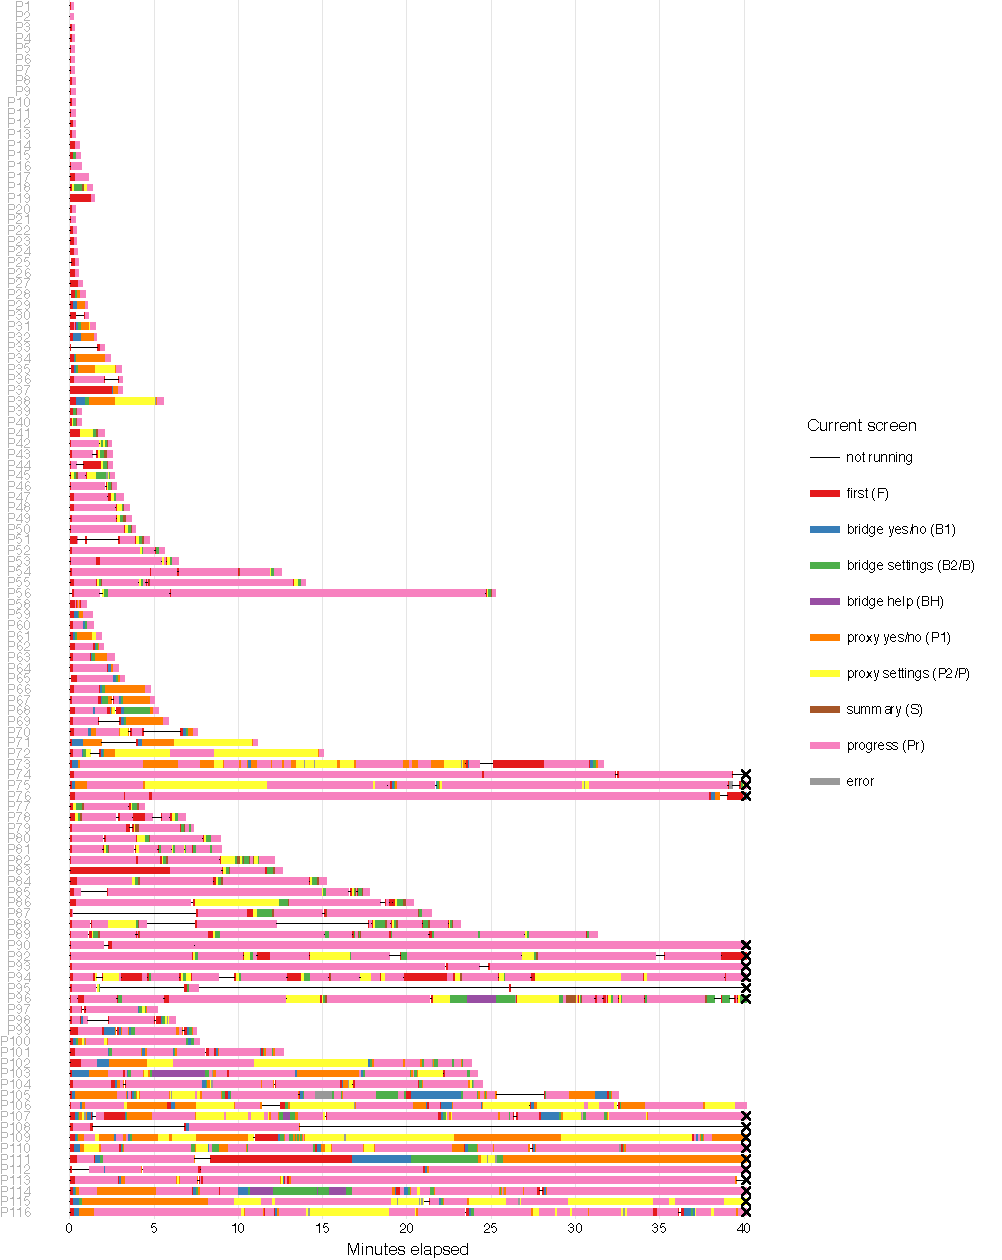
\includegraphics{all-participant-edges}
\caption{
A summary of our valid participants' paths through the interface.
The length of the bars show the total time taken to complete the task,
except for those we cut off after approximately 40 minutes.
Different colors indicate which screen they were on during the experiment.
The ``not running'' times are those when Tor Launcher was closed (
i.e. searching for help in another browser, restarting the application, etc.).
}
\label{fig:all-participant-edges}
\end{figure*}

\subsubsection{Completion Rate} 

%table
\begin{table}[t]
\centering
% Do not edit this file. Edit attempts.R instead.
\begin{tabular}{r c c c c c c}
& \rotatebox{90}{E1-NEW} & \rotatebox{90}{E1-OLD} & \rotatebox{90}{E2-NEW} & \rotatebox{90}{E2-OLD} & \rotatebox{90}{E3-NEW} & \rotatebox{90}{E3-OLD} \\
no bridge, no proxy & 17 & 13 &  &  &  &  \\
obfs3, no proxy & 2 & 6 & 18 & 16 &  &  \\
meek-amazon, no proxy &  &  &  &  & 7 & 4 \\
meek-google, no proxy &  &  &  &  & 5 & 4 \\
meek-azure, no proxy &  &  &  &  & 1 & 1 \\
no bridge, 3rd-party proxy &  &  &  &  &  & 1 \\
DNF (did not finish) &  &  &  & 3 & 6 & 10 \\
\end{tabular}

\caption{
Network components that led to the first successful bootstrap
in each condition.
Most successful E1 participants used a direct connection,
but a few optionally used an obfs3 bridge.
All successful E2 participants used 
an obfs3 bridge (the recommended option)---none used 
flashproxy, fte, fte-ipv6, obf4, or scramblesuit bridges to connect. 
Most successful E3 participants
used a meek bridges, disfavoring meek-azure.
One E3 participant succeeded in an unexpected way
by using an open proxy and configuring it to bypass our 
simulated environment.
}
\label{tab:attempts-bridge-proxy}
\end{table}

%overview
Completion rate was defined as the percentage of users that eventually connected to Tor. Table~\ref{table:participant-summary} summarizes the completion rates and Table~\ref{tab:attempts-bridge-proxy} shows the configuration for users' first successful connection. We only considered the first successful configuration, as some curious participants tried others after completing their task. 

% failure observations
17\% (19 of 114) of participants were not able to successfully connect to Tor. Five (P73, P75, P89, P91, P106, P110) tried a direct connection. When that failed, they assumed there was something wrong with their computer, network settings, or the Tor network and never tried to configure bridges or proxies. Five (P74, P92, P105, P107, P113) users who need a bridge assumed that they needed a proxy to connect to Tor. We belive this may be due to the fact that the OLD interface defaults to showing users the proxy page (because it is the one before the progress screen) when a connection fails. Five (P90, P93, P108, P111, P114) users who needed a meek or custom bridge tried the suggested bridge (obfs3), but didn't know what to do when that failed. Two (P94, P109) users who needed a meek or custom bridge tried to get custom bridges but failed to format their email content correctly to get a response from the bridges autoresponder. We suspect that they would have succeeded if they had gotten a response. 

%success rate and version
Our interface changes did {\it not} have a significant impact on completion rates (Pearson's Chi-squared; $X^2 = 0.0126$, $df = 2$, $p = 0.994$). That is, the slight differences in completion rates between E1-NEW vs E1-OLD, E2-NEW vs E2-OLD and E3-NEW vs E3-OLD are likely due to random chance.

\subsubsection{Connection time} 
Connection time is the time from Tor Browser starup to the first successful Tor bootstrap. Non-finishing participants are assigned the maximum experiment time of 40:08. Table~\ref{table:participant-summary} summarizes the median times while Figure~\ref{fig:time_to_success_clamped} shows their distribution. Figure~\ref{fig:time_to_success_ecdf} shows the cumulative success rates over time. 

%time observations (how long people took)
The simulated censorship environment, and therefore, the difficulty of the configuration, was the most determining factor for connection time (Kruskal--Wallis $\chi^2 = 80.5$, $\mbox{df} = 2$, $p < 10^{-15}$). Participants in E2 took longer to connect than participants in E1, and participants in E3 took the longest to connect.

%time to success and version
Our interface changes had a significant impact in reducing connection time (one-tailed Mann--Whitney; $ Z = -1.84$, $p = 0.0328$, $r= 0.172$). That is, the differences in mean connection times in E1-NEW vs E1-OLD and E2-NEW vs E2-OLD and E3-NEW vs E3-OLD is likely not due to random chance. We used a one-tailed Mann--Whitney test because the distribution of completion times were 1) right-censored at 40 minutes (experiment duration) and 2) non-normal and heavily right tailed (failures were assigned a time of 40 minutes). 

\begin{figure}[t]
\centering
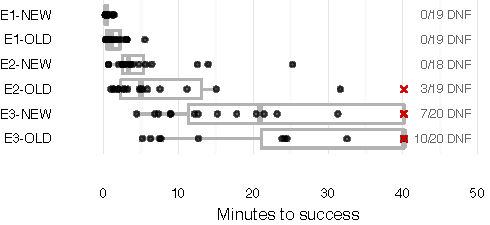
\includegraphics{time_to_success_clamped}
\caption{
The dots show the raw connection times,
while the boxplots show the medians and interquartile ranges.
The ``DNF'' (did not finish) numbers at the right show how many of participants 
did not finish, who were assigned the maximum time of 40:08.
}
\label{fig:time_to_success_clamped}
\end{figure}

\begin{figure}[t]
\centering
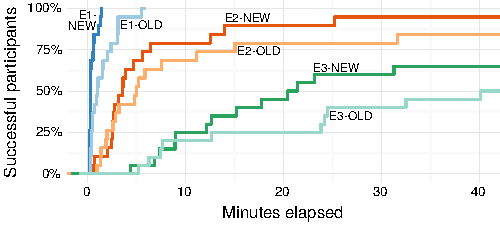
\includegraphics{time_to_success_ecdf}
../experiment/processing/time_to_success_ecdf.tex
\caption{
Cumulative success rates over time, shown continuously and at discrete times we found interesting.
For the purposes of plotting the cumulative distribution, those who did not finish were assigned
an arbitrarily high number greater than 40 minutes. 
Notice that the longer the time went on, participants were less likely to succeed. 
At 1.5 minutes, every E1-NEW participant finished,
but only 58\% of E1-OLD had finished by that time.  
At 10 minutes, most participants in E2 had finished. 
}
\label{fig:time_to_success_ecdf}
\end{figure}


\subsubsection{Configuration Time} 
Configuration time is the time spent configuring network components, which we define as the completion time minus any time spent on the progress screen. Table~\ref{table:participant-summary} shows the median times and Figure~\ref{fig:time_to_success_active_clamped} shows their distribution. Table~\ref{table:median_time} shows the percentage of time spent on each screen. Note that the time spent configuring bridges and proxies is {\it not} equivalent to the amount of time participants spent trying to connect, which would be the connection time minus the time spent on the progress screen for the last time (time Tor takes to bootstrap after a valild configuration). 

%things to keep in mind
We believe that configuration time is a meaningful metric because 1) bootstrapping can take a couple minutes, which dominates measurements for users do not need much time to configure their connection, such as participants in E1. and 2) some mistakes, such as using a syntactically valid but unsuable proxy, generate non-interruping warnings and let the users wait indefinitely at until they manually cancel the connection to try again. But this is not the most accurate measurement of time spent configuring, since it does not reflect how some participants searched for help in another browser while waiting on the progress screen.

%configuration time and version
Our interface changes had a significant impact in reducing configuration time (one-tailed Mann--Whitney; $Z = -3.28$, $p = 0.000516$, $r = 0.307$). That is, the differences in mean configuration times in E1-NEW vs E1-OLD and E2-NEW vs E2-OLD and E3-NEW vs E3-OLD is likely not due to random chance. We used a one-tailed Mann--Whitney test because the distribution of configuration times were also 1) right-censored and 2) non-normal and heavily right tailed, due to being an artifact of completion time. 

\begin{table}[t]
\centering
\begin{tabular}{l r r r r}
& First & Proxy & Bridge & Progress \\
\noalign{\hrule}
E1-NEW & 28\% & 0\% & 0\% & 60\% \\
E1-OLD & 30\% & 0\% & 0\% & 29\% \\
E2-NEW & 6\% & 5\% & 6\% & 78\% \\
E2-OLD & 7\% & 18\% & 8\% & 45\% \\
E3-NEW & 3\% & 5\% & 5\% & 77\% \\
E3-OLD & 2\% & 12\% & 6\% & 64\% \\
\end{tabular}

\caption{The median percent of time spent on each screen, which is not
necessarily the median absolute time spent on that screen. 
This percentage is computed independently for each screen; that is, a participant who spent the median percent 
of time on one screen may not be the same participant who spent the median percent
of time on other screens.} 
\label{table:median_time}
\end{table}

\begin{figure}[t]
\centering
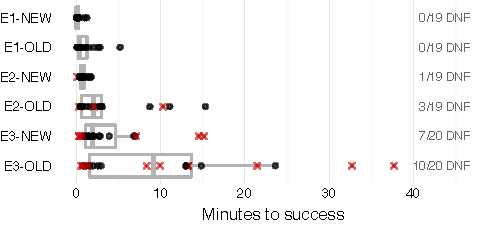
\includegraphics{time_to_success_active_clamped}
\caption{
The dots show the raw active configuration times,
while the boxplots show the medians and interquartile ranges.
Here, non-finishing participants' active time was computed by
subtracting the amount of time spent on the progress screen from the 
their assigned completion time of 40:08.
}
\label{fig:time_to_success_active_clamped}
\end{figure}

\subsection{Usability of Tor Launcher} 
In total, 63\% (72 of 114) of first attempts to connect failed and 79\% (363 of 458) of total attempts to connect failed. 
On average, users who required a bridge took over 3 minutes to connect to Tor, and users who required a meek or cutsom bridge took over 20 minutes.

Ideally, almost all users should be able to configure the necessary or optional network components and connect to Tor within a few minutes. Neither the Tor Browser's 5.0.3. Tor Launcher GUI or our redesigned Tor Launcher GUI meets this goal.

\section{Recommendations}
\label{recommendations}
We do believe that adopting our design will help save users time when connecting to Tor. But since we did not test our design changes independently, we cannot (and do not) claim the effects each change we made. Therefore, we do not recommend specific changes, but offer some suggestions for Tor Launcher's GUI based on what we learned: \\

\begin{itemize}
\item {\bfseries Use less words.} Shorten text so users read it.
\item {\bfseries Give advice.} Discourage users from configuring optional components. Add a secondary recommendation (try meek if obfs3 doesn't work). 
\item {\bfseries Hide infrequent options.} Hide the proxy configuration screen and less-used transports. 
\item {\bfseries Minimize work.} Detect if users need a proxy or not. Redirect users to the relevant pages on error (i.e. redirect to the bridge screen the bridge fails).  
\item {\bfseries Add system visibility.}  Show users their bridge and proxy settings before and during connection. Fix the progress bar updating weirdness.
\item {\bfseries Provide feedback.} Tell users what to do when a specific error occurs (i.e. try agin, fix bridges, etc.). 
\end{itemize}

We also recommend exploring solutions that leverage automation, user-dependent inputs, or network-dependent inputs. We start this discussion by sharing some of our own ideas in appendix~\ref{alternatives}. 

\section{Limitations}
\label{sec:limitations}
We did not study international users, or the configuration interface in languages other than English. All of our participants were from the United States and instructed to interact with the English version of Tor Browser.

Participants in a laboratory setting may alter their due to their awareness of being observed~\cite{mccarney2007hawthorne}. We are aware that our participants were likely motivated differently compared to real users. We believe that participants were likely overmotivated to connect to Tor because they were being observed and recieving a monetary reward. If true, this makes our results are a conservative estimate of the current usability problems. 

Since the configuration interfaces in simulated environments, we cannot claim how difficult it would be for a user to connect to Tor in a certain country or how much our redesigned interface would help those users.  

Our experiment did not directly test more advanced tasks. Our simulated environments did not require users to configuring a proxy or to get a custom bridge. From observing of user attempts to configure proxies and get custom bridges, we suspect users generally struggle with these tasks but cannot quantify how much they do. 

We only tested interface on Windows machines, which were the machines available at <redacted>. %Xlab.
The configuration interface leverages the native operating system's styling and elements, making the configuration interface on Windows look slightly different from the OSx or Linux equivalent. Additionally, we acknowledge that participants' unfamilarity with Windows may have affected our experiment, but we believe that this affected all experimental conditions minorly and equally.  

\section{Related Work}
\label{sec:related} 

{\color {red} 
There have been three published user studies on Tor. Clark et~al.~\cite{clark2007usability} examined various deployment
options for Tor Browser, such as Vidalia, Privoxy, Torbutton, and FoxyProxy, and found that none had satisfactory from a usability. Fabian et~al.~\cite{fabian2010privately} show that Tor's added
latency~\cite{dingledine2009performance} causes users
to be frustrated, cancel requests, and prevents user adoption. 
Norcie et~al.~\cite{norcie2012eliminating} found found that 
64\% of users are unable to continue with installation or browsing at least once due to difficulties.

We do not know of any published usability evaluations of
Tor Browser since the release of the 3.5 series in 2013, which introduced radical UI changes~\cite{torbrowser-35}.
The most recent effort is an unpublished pilot study by Lee and Fifield~\cite{uxsprint} 
that tested the downloading, installation, and browsing tasks in Tor Browser.  This study uncovered a number of issues~\cite{uxsprint2015-tickets},
some of which influenced changes in Tor Browser version~4.5 and later.

Previous user studies have considered the whole browsing experience,
without focusing on specific features in isolation.
Our study focuses on 
the browser's configuration interface, which guides users through setting up components required to circumvent censorship. 
%for color red
}

\section{Conclusion} 
\label{sec:conclusion}

{\color {blue}
We conducted a series of experiments to improve the Tor Browser 5.0.3 configuration interface. A couple sentences to summarize the whole thing. Echo roadmap in intro, but make it summary-like. 

%proof that user testing is important and general advice to for more research on Tor
Tor doesn't collect any information or perform AB testing, so this type of user research is especially important. to set it up, get users, computers, consent, and instrumented versions of the software. Research can be exploratory (ask users what they want), observational (look at what they do), or testing a hypothesis (verify changes). We encourage the use of simulated censorship environments as a tool for user testing censorship circumvention software. Not only do simulated environments avoid rerouting traffic through a censoring country's networks, their reproducibility and stability are ideal for experiments. 
}

\section {Experiment Artifacts} 
Due to space constraints, we could not include many of our experiment artifacts. This includes the experiment setup and teardown code, firewall rules that simulated censorship environments, interview transcriptions from the formative user study, logs from our instrumented configuration interfaces, and videos of users attempting to connect to Tor through the configuration interface. We urge you to check out the project repository: \\

\noindent <redacted url>
%\noindent \url{https://github.com/lindanlee/circumvention-ux-tor}

\section {Acknowledgments}
Many generous people helped us along the way. <Redacted> assisted with testing our setup and teardown scripts, offered recruitment services, and allowed us to run experiments after <redacted lab>'s hours. <Redacted> and <redacted> were instrumental during the design process, as they helped me interate through many not-so-great ideas.  <Redacted>,and <redacted> provided me with insider insight into the design decisions made at Tor.
% Rowilma del Castillo. Nima Fatemi and Isabela Bagueros.  Georg Koppen and the Tor UX team.

\bibliographystyle{abbrv}
\bibliography{pets2017-paper}

\appendix

\section{Success and Error States in Tor Launcher 5.0.3} 
\label{states} 
{\color {blue} 
A reminder of the digraph, and a reference (Figure~\ref{digraph}). Give an example of one input leading to many end states. 

% e12; selected proxy type, good address syntax, good ip address, blank port (bridge) 
% s2; selected proxy type, good address syntax, good ip address, blank port (bridge)
% e12'; selected proxy type, good address syntax, good ip address, blank port (no bridge)
% s2'; selected proxy type, good address syntax, good ip address, blank port (no bridge)

success states: 
\begin{itemize}
\item s0: no bridge no proxy connection.
\item s1: bridge, no proxy connection.
\item s2: bridge and proxy connection (correct proxy syntax and with default port)
\item s3: bridge and proxy connection (correct proxy syntax and with specified port)
\end{itemize}

error states:
\begin{itemize} 
\item e0: custom bridge: field left blank
\item e1: custom bridge: syntax error
\item e2: custom bridge: good syntax, bad ip address
\item e3: hardcoded bridge: bridge blocked in country
\item e4: bridge blocked in country
\item e5: blank proxy input
\item e6: no proxy type
\item e7: selected proxy type, bad address syntax
\item e8: selected proxy type, good address syntax, bad ip address, blank port
\item e9: selected proxy type, good address syntax, bad ip address, good port
\item e10: selected proxy type, good address syntax, bad ip address, bad port
\item e11: selected proxy type, good address syntax, good ip address, bad port
\item e12: selected proxy type, good address syntax, good ip address, blank port
\end{itemize} 
}

\section{Qualitative User Study Recruitment Posting} 
\label{qualitative-recruitment}
We are recruiting participants for an in-person research study at <redacted>. %the University of California, Berkeley. 
You will need to come in to our lab and perform tasks on a computer for an hour or less. You will be compensated \$30 for participating. 
No special knowledge and no technical experience is required. If you are interested, fill out the survey at \textit{<survey link>}. 

\section{Qualitative User Study Prescreening Survey} 
\label{qualitative-prescreening}
We are recruiting participants for an in-person research study at the <redacted>. %University of California, Berkeley. 
You will need to come in to our lab and perform tasks on a computer for an hour or less. You will be compensated \$30 for participating. No special knowledge and no technical experience is required.\\

\begin{enumerate}
\item{Please select when you are available. We will assign you an hour experiment time slot during one of those times.}
\item{I am able to provide my own transportation to the <redacted> %University of California, Berkeley 
campus.}
\item{Thank you for your interest! Please provide an email address where we can contact you to share more logistical details.}
\item{we are looking for a very small number of participants, so unfortunately, we may not be able to accommodate everyone who applies. Would you like us to let you know about future opportunities?}
\item{What is your gender?}
\item{What is your age?}
\item{Please select your highest completed (or current) level of education.}
\item{What is your occupation?} 
\item{Do you speak any languages other than English fluently?}
\item{If you have a personal computer, what kind do you use?}
\item{Which of the following terms have you heard of? \textit{<answer choices: a checkboxlist of the the following terms: malware, proxy services, phishing, SSL, X.511 certificates, Tor>}}
\item{How often do you use the following software or features? \textit{<answer choices: a grid of radio buttons. Software/features (rows): HTTPS on web pages, proxies or other censorship circumvention tools, virtual private networks (VPN), file or whole-disk encryption, anonymity systems (e.g., Tor), email encryption (e.g., PGP), chat or instant messaging encryption, voice communication encryption. Frequency (columns): never, less than once a month, a few times a month, several times a week, daily.>}}
\end{enumerate}
Thank you for filling out this form. You are now done!

\section{Prescreening Survey Responses}
\label{prescreening-responses}
{\color{blue} 
short intro and conclusion. Take self-reported with a grain of salt, but here they are anyways. 

\begin{figure}[t]
\centering
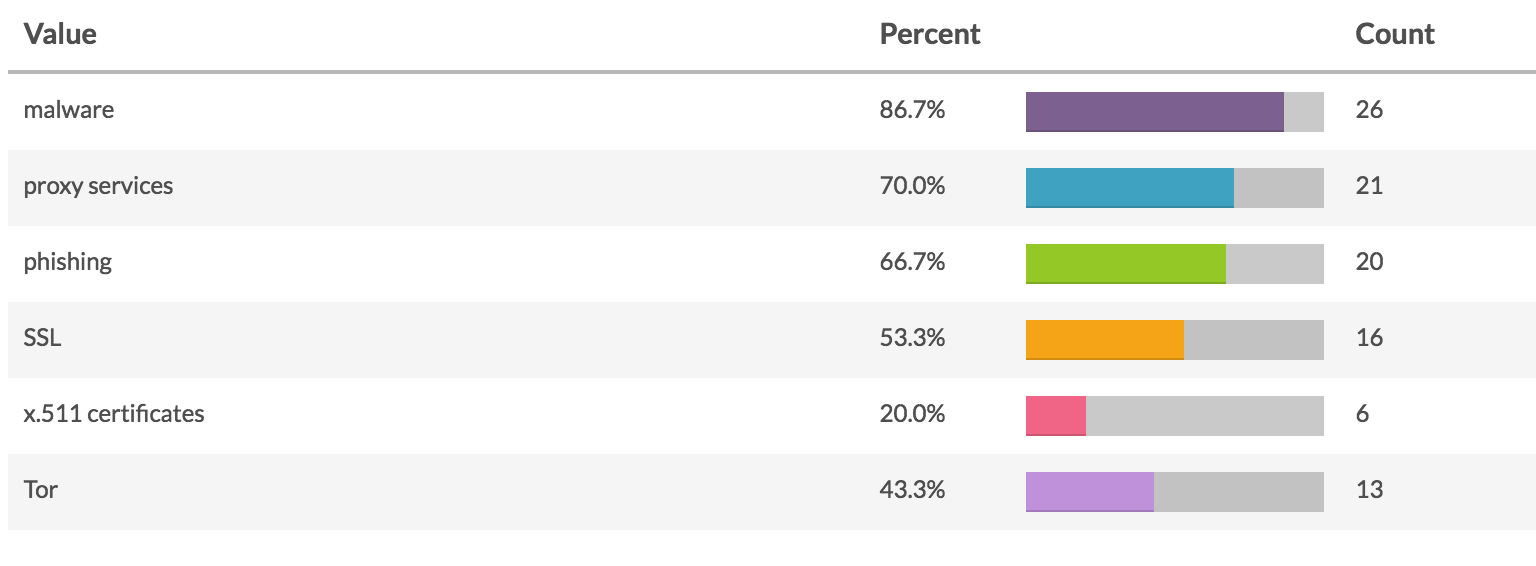
\includegraphics[width=.5\textwidth]{self-reported-tech-familiarity.png}
\caption{most participants reported familiarity with terms, even made up ones.}
\end{figure}

\begin{figure}[t]
\centering
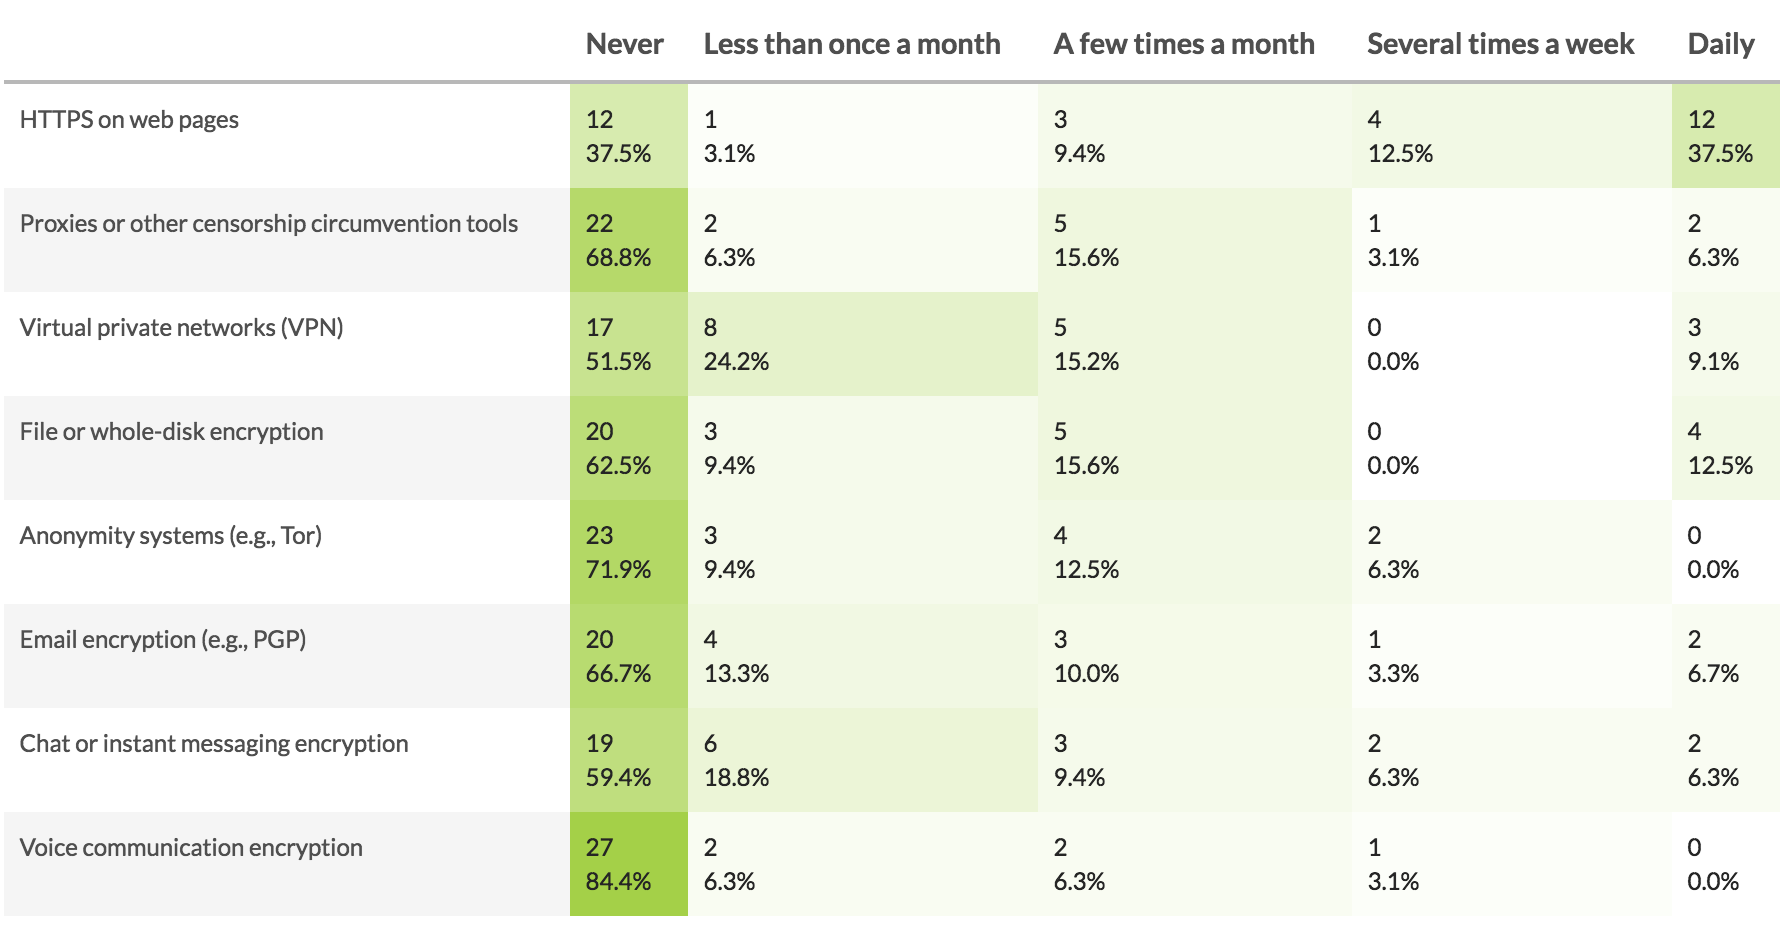
\includegraphics[width=.5\textwidth]{self-reported-security-use.png}
\caption{most people didn't use many security tools.}
\end{figure}
}

\section{Qualitative User Study Introduction Script} 
\label{qualitative-script} 
Imagine you live in an oppressive country that censors part of the Internet. We have simulated this in the laboratory by blocking certain websites and services.  The purpose of this experiment is to evaluate the use of Tor browser, which is a browser that can circumvent censorship and let you visit blocked websites. Currently, torproject is blocked (you can check this by going to torproject.org on a standard browser, like Firefox, Chrome, or Internet Explorer). 

To circumvent censorship successfully, you will need to set up Tor browser correctly and use it to get to Wikipedia. If you are able to reach the website, then you know that you have successfully circumvented censorship. Fill out the question on the worksheet. This isn't intended to be hard, just write what you see. We want to just check you saw the website. 

Before you start, do you have any questions about what you are asked to do? 

\section{Participant Worksheet Text} 
\label{participant-worksheet}
Imagine you live in an oppressive country that censors part of the Internet. We have simulated this in the laboratory by blocking certain websites and services. The purpose of this experiment is to evaluate the use of Tor browser, which is a browser that can circumvent censorship and let you visit blocked websites. For instance, www.torproject.org is blocked. Check this by going to the site on a standard browser, like Firefox, Chrome, or Internet Explorer. It will fail to load, when you can visit other sites.

To complete this worksheet, you will need to set up Tor browser (on your desktop) correctly and use it to get to blocked site. If you can visit wikipedia, then you know that you have successfully circumvented censorship.

\section{Post-Experiment Standard Interview Questions}
\label{interview-questions}
We asked our participants these questions after they were given time to configure Tor Browser. \\

\begin{enumerate}
\item{Can you talk us through what you did along with what you were thinking at the time?}
\item{What was most challenging part of connecting?}
\item{Were there any unfamiliar terms?}
\item{How did you decide which options to choose?}
\item{What did you think about using Tor?}
\item{What is one change you would recommend?} 
\item{Did you need any additional information?} 
\end{enumerate}  

In addition to these questions, we asked our participants about specific questions based on their observation, usually regarding a specific choice in action, a particular screen they seemed stuck on, and any errors they encountered during the configuration process. 

\section{Quantitative User Recruitment Posting}
\label{quantitative-recruitment}
We are recruiting up to 40 participants for a user study at <redacted>. %UC Berkeley. 
The experiment will involve basic Internet browsing tasks. You are not eligible if you have participated in our previous sessions.\\

\indent Payment: \$30 Amazon gift card\\
\indent Duration: 1 hour \\
\indent Where: <redacted> \\ %Xlab at Hearst Memorial Gymnasium\\

\textit{<list of sessions>}\\

To be eligible, you must be an adult (18 or older). This is to comply with university policies on research. 

If you are interested: 1. Email <redacted> %lnl@berkeley.edu 
with the sessions you are able to attend. We will confirm your participation and assign you a session. 
2. Come to <redacted> %Xlab 
at the appointed time for the experiment.

\section{Quantitative User Study Introduction Script} 
\label{quantitative-script} 
Imagine you live in an oppressive country that censors part of the Internet. We have simulated this in the laboratory by blocking certain websites and services.  The purpose of this experiment is to evaluate the use of Tor browser, which is a browser that can circumvent censorship and let you visit blocked websites. Currently, torproject is blocked (you can check this by going to torproject.org on a standard browser, like Firefox, Chrome, or Internet Explorer). 

To circumvent censorship successfully, you will need to set up Tor browser correctly and use it to get to Wikipedia. Tor is already installed for you. On the desktop, you should see a globe icon that says ``Start Tor Browser.'' If you are able to reach the website, then you know that you have successfully circumvented censorship. Fill out the question on the worksheet. This isn't intended to be hard, just write what you see. We want to just check you saw the website. 

Afterward, we ask you to take a short survey to collect some information about you. The link is also on your worksheet.
We will give you time to complete this task. If you finish early, we ask that you sit at your desk until the remainder of the hour. Since we are recording your screen, we ask that you don't do anything personal afterward, like checking your email.

Before you start, do you have any questions about what you are asked to do? 

\section{Quantitative User Study Exit Survey} 
\label{quantitative-exit-survey}
We'd like to know more about you.  All of your answers will be stored separately from any identifying information in order to protect your confidentiality.

This survey is part of a research project being conducted by the <redacted>. %University of California, Berkeley. 
If you have any questions about your rights or treatment as a research participant in this study, please contact the <redacted>'s %University of California at Berkeley's 
Committee for Protection of Human Subjects at 510-642-7461, or email 
<redacted>. %subjects@berkeley.edu. 
If you agree to participate, please click Next below.\\

\begin{enumerate}
\item{What is your participant ID? (This can be found on the sticker on the left hand corner of the desk you are currently sitting at.)}
\item{What is your gender?}
\item{What is your age?}
\item{Please select your highest completed (or current) level of education}.
\item{What is your current occupation?}  
\end{enumerate}

Thank you for participating in our experiment. You are now done! Please sit at your desk for the remainder of the experiment. Our researchers will formally announce the end of the experiment. 

\section{Alternative Approaches} 
\label{alternatives}
{\color {blue}
Our goal was to deploy impactful, tested changes the Tor configuration interface. In fact, Tor version~4.5 incorporated textual and navigational changes based on our redesigned interface. Throughout our experiments, we collaborated with Tor developers and focused on discovering changes that could be deployed right away. For this reason, we assumed that the configuration process will remain a manual process that requires user inputs, as it is currently deployed. However, we list some alternative approaches that seem worth exploring. \\

%remember: 	no user inputs, no network inputs, minimize info leaks
%and:		minimal user work, full user control 

\begin{description}
\item{\bfseries Automate the configuration.} The most efficient way to connect as many users to the Tor network is to automatically configure their connection on start. A naive automation is to try configurations that would most likely work, in order (i.e. a direct connection, then an obfs3 connection without a proxy, then an meek bridge connection with out a proxy). This leaks to network eavesdroppers that the user is connecting to the Tor network. We do not know how much risk is associated with this approach. 
\item {\bfseries automate after the first failure.} The network leak happened. But then this automation would be pretty fingerprintable behavior. 
\item{\bfseries Ask about the risk.} An alternative to naive automation is to offer manual configuration to those that want to be more cautious and automatically configuring a connection for who are not at risk. The complication with this approach is that users may not be qualified to answer if they are at risk or may not trust Tor with this information. 
\item{\bfseries Ask if users know what to do.} Another alternative to naive automation is to offer manual configuration to those that know how to configure their connection and to automate the process for users who do not know how to configure their connection. This may prevent the most mistakes, but does not account for the users' risk associated with using Tor. 
\item{\bfseries Suggest configurations.} A way to help users without any automation or questions is to give users information about what would work in their country. The first page of the configuration interface can show a list of countries with a corresponding recommended configuration. This approach does not require users to answer about their risk, technical ability, or location. However, it does require that the user trust the given advice and to correctly configure their settings based on this advice. 
\item{\bfseries Assign configurations.} This is a smart way to automate connections to the Tor network. Upon start, the interface detects proxy settings and uses them, if any. Then, all users connect to bridges that will always work (such as meek bridges), which assign them a guard relay based on their location, effectively assigning bridges for the user. 
\end{description}

We believe that automation, asking about risk, and identifying struggling users could enable significant improvements to the configuration process. 
}


\end{document}
